%! TEX root = ../main.tex
\chapter{研究设计}\label{chap:3}
\section{样本选择与数据来源}
\subsection{极端天气样本与数据}\label{sec:def}

气候代表了一个地区在一定时间跨度内所经历的天气状况的总体特征,揭示了一个地区的基本气象冷热、干湿特性,故而温度和降水是构成某一地区气候特征的两个最根本的气象要素\citep{alexander2006global}。在气候变化的大背景下,异常气候以及极端天气事件发生的可能性增加\citep{aigner2023summary,donat2017addendum},这其中极端强降水愈发频繁\citep{trenberth2010relationships}。在我国,极端天气事件如洪涝、台风、暴雪等自然灾害\citep{尹红2019基于},往往与极端强降水事件密切相关,给国家和人民带来了巨大的损失。因此,本文选取将极端降水作为极端天气事件的代表来,数据来源于国家气候中心,时间范围为1954年至2019年。

对于极端降雨强度的定义,国家标准 GB/T 33680-2017《暴雨灾害等级》中将日降水量超过 50mm 定义为暴雨,超过100mm定义为大暴雨,超过 250mm 定义为特大暴雨。然而,由于不同地区在气候特征和降水模式上存在显著差异,单一的数值标准可能无法全面反映极端降水事件的影响。参考国际气候变化检测和指数专家组(ETCCDI)采用分位数来定义极端天气的方法,将日降水量超过95th或99th百分位数的情况定义为极端降水\footnote{资料来源:UVIC,\url{https://etccdi.pacificclimate.org/list_27_indices.shtml}}。这种方法能够更好地适应不同地区的降水特征\citep{karl1999clivar},因此本文选择将极端降水天气定义为20年一遇的降水天气。
% 年遇类型只是一个概率的问题,年度发生的概率是1/20,对应95的分位数
\begin{figure}[H]
    \begin{minipage}{0.48\linewidth}
        \centering
        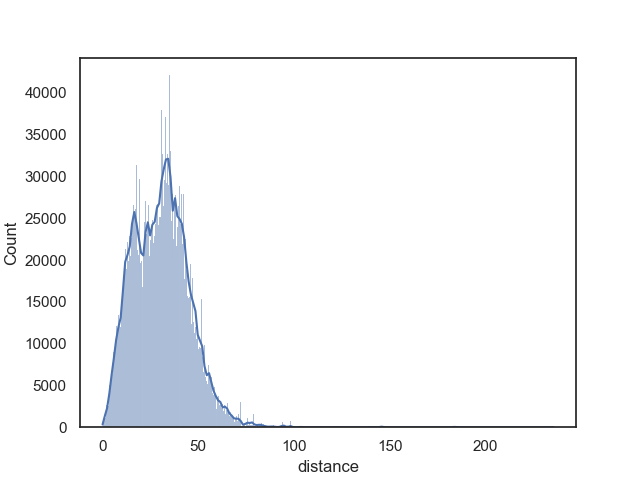
\includegraphics[width=\textwidth]{lib/img/distance.png}
        \caption{保险标与最临近气象站距离分布(千米)}
        \label{fig:distance}
    \end{minipage}
    \begin{minipage}{0.48\linewidth}
        \centering
        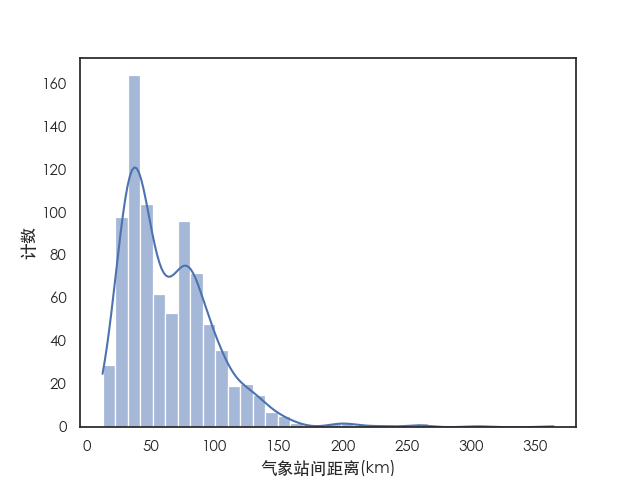
\includegraphics[width=\textwidth]{lib/img/locations_distance.png}
        \caption{气象站间距的地理位置分布(千米)}
        \label{fig:locations}
    \end{minipage}
\end{figure}

而关于极端降雨受灾范围的界定,结合降水数据和保单数据(见\ref{sec:data}),考虑到绝大多数保险标的与距离最近的气象站之间距离大多在50公里以内,平均距离不足30公里,如图\ref{fig:distance},因此本文将距离监测到极端降水的气象站20公里内的区域定义为灾区。而考虑到我国气象站分布间距基本在100公里以内,如图\ref{fig:locations},因此取气象站所覆盖的受灾半径最多为50公里,定义距离监测到极端降水的气象站20-50公里内的区域为近灾区,50公里以上的区域为远灾区。而如果近灾区/远灾区标的在过去投保时曾经历降水冲击则将该标的去重。

气象站地理位置分布如图\ref{fig:location}所示。

\begin{figure}[H]
    % \centering
    % \begin{minipage}{0.48\linewidth}
        \centering
        \includegraphics[width=0.8\textwidth, trim=200 0 200 0]{lib/img/locations.png}
        \caption{所有气象站的地理位置分布}
        \label{fig:location}
    % \end{minipage}
%     \begin{minipage}{0.48\linewidth}
%         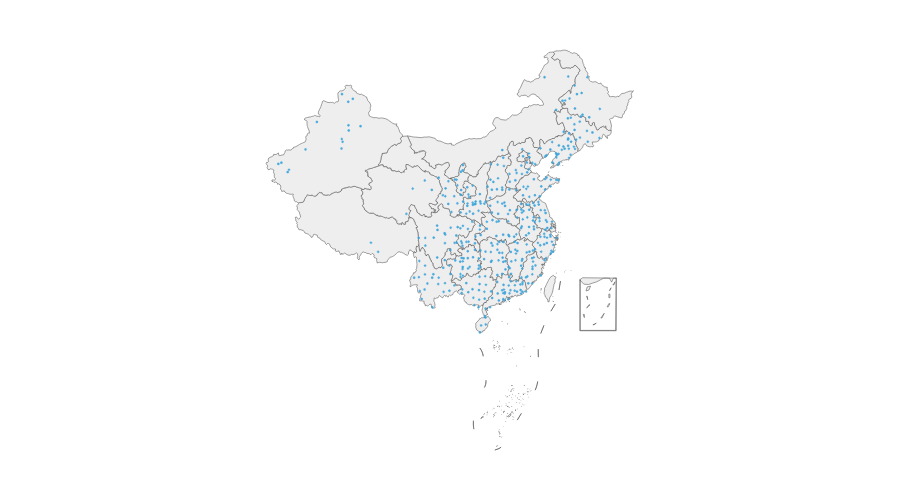
\includegraphics[width=\textwidth, trim=200 0 200 0]{lib/img/near.png}
%         \caption{划分为灾区气象站的地理位置分布}
%     \end{minipage}
% \end{figure}
% \begin{figure}[H]
%     \begin{minipage}{0.48\linewidth}
%         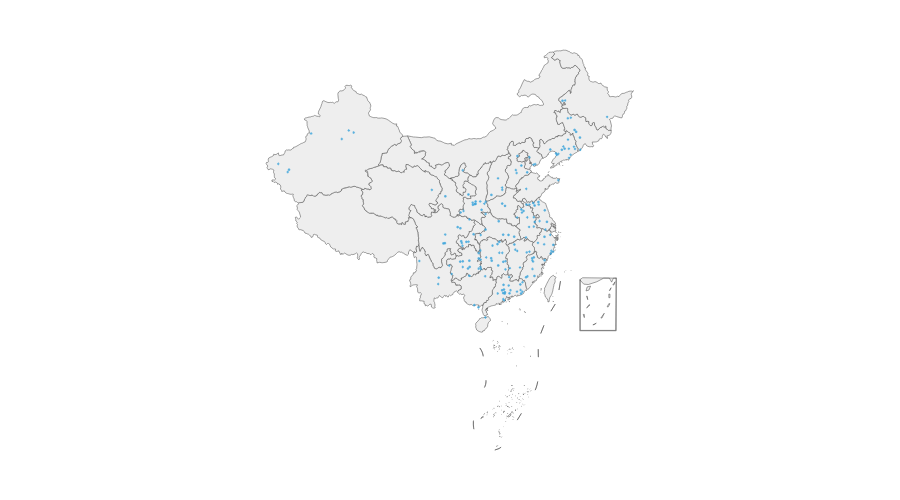
\includegraphics[width=\textwidth, trim=200 0 200 0]{lib/img/middle.png}
%         \caption{划分为近灾区气象站的地理位置分布}
%     \end{minipage}
%     \begin{minipage}{0.48\linewidth}
%         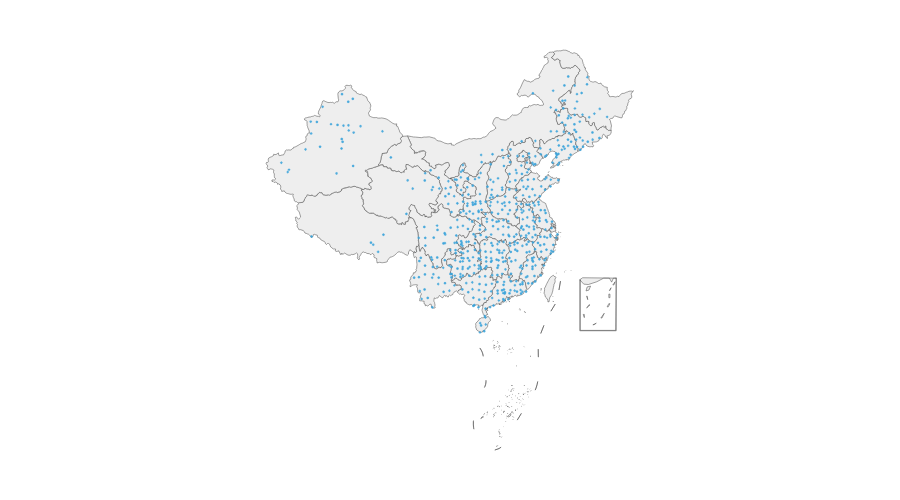
\includegraphics[width=\textwidth, trim=200 0 200 0]{lib/img/far.png}
%         \caption{划分为非灾区气象站的地理位置分布}
%         \label{fig:end}
%     \end{minipage}
\end{figure}
\subsection{保险标的样本与数据}\label{sec:data}
本文以某财产保险公司1995年1月1日至2015年12月31日全国家财险承保理赔数据作为研究样本。

为了确保气象数据与标的样本之间的相关性,对样本基于距离进行了筛选,只选择了那些距离最近的气象站20公里以内的标的样本,并剔除存在指标为空值等的异常值,然后再进行灾区、近灾区和非灾区划分进行分析并去重,共有约37万条数据。为降低异常值影响,本文对所有连续变量进行了1\%缩尾处理。

\section{模型设定与变量选取}
\subsection{变量定义}
本文选取户均保额作为被解释变量。主要解释变量为样本是否在灾区或者近灾区,以及是否在极端降水冲击后。

为了更清晰地评估降水冲击的影响,本文纳入一系列控制变量。这些变量包括:

\begin{enumerate}
    \item 是否历史投保:该保险标的是续保还是首次投保,续保的保险标的可能更倾向于保额覆盖更高的保险
    \item 保险财产的购置价:反映了家庭财产的价值,通常财产价值越高,对风险的担心也越大,保险需求也越大。
    % \item 建筑面积:建筑面积越大,需要更高的保险保额来覆盖潜在的风险。
    \item GDP增速:反应当地经济增长率,经济增长会促进保险购买。
    \item 保险深度:反映了当地保险市场的发展程度,保险市场发展程度越高,家庭购买保险的可能性也越大。
\end{enumerate}

被解释变量与控制变量含义如表\ref{tab:var}所示。
\begin{table}[H]
    \caption{变量定义表}\label{tab:var}
    \centering
    \begin{tabular}{@{}cccc@{}}
        \toprule
        变量类别                    & 变量名称         & 变量定义    & 变量解释                \\ \midrule
        被解释变量                   & Coverage     & 保额      & 保险金额                \\ \midrule
        \multirow{3}{*}{主要解释变量} & Disaster     & 灾区      & 是否处于极端降水监测点20公里内    \\ \cmidrule(l){2-4}
                                & Neighbor     & 近灾区     & 是否处于极端降水监测点20-50公里内 \\ \cmidrule(l){2-4}
                                & Post         & 降水发生时间  & 是否在极端降水发生后投保        \\
        \midrule
        \multirow{3}{*}{控制变量}   & Prem\_before & 历史投保    & 保险标的是否有投保记录         \\ \cmidrule(l){2-4}
                                & Price        & 保险财产购置价 & 保险标的资产购置价           \\ \cmidrule(l){2-4}
                                & Area         & 建筑面积    & 保险标的建筑面积            \\ %\cmidrule(l){2-4}
        % & Claim       & 是否理赔    & 该保单是否发生理赔            \\
        \bottomrule
    \end{tabular}
\end{table}


\subsection{模型设定}
极端天气事件是一个外生冲击,在时空上的分布是随机的,因此本文采用了DID回归来估计极端天气事件对家庭财产保险的影响。本文设定实验组和对照组,实验组为受灾区或近灾区,对照组为未受灾区。

针对假设\ref{hyp:3},本文建立双重差分模型\ref{eq:DID_1}
\begin{equation}
    \log\text{Coverage}_{it}=\alpha+\beta_1\text{Neighbor}_{i}+\beta_2\text{Post}_{it}+\beta_3\text{Neighbor}_{i}\times\text{Post}_{it}+\beta\text{Controls}_{it}+\varepsilon_{it}
    \label{eq:DID_2}
\end{equation}

其中,$\text{Coverage}_{it}$为家庭$i$的家财险保额,用来表征家财险需求。家庭$i$表示某场极端降水冲击下的某家庭,$t$指代极端降水冲击的年份。$\text{Neighbor}_{i}$为家庭是否位于近灾区,近灾区家庭为处理组,取值为 1;远灾区家庭为对照组,取值为 0。$\text{Post}_{it}$为家财险生效时间是否在极端天气事件后,冲击后一年内为1,冲击前一年为0。$\text{Neighbor}_{t}\times\text{Post}_{it}$为交互项,其系数反映了单次极端天气冲击对近灾区家庭家财险需求的平均因果效应,$\text{Controls}_{it}$为控制变量,包括是否历史投保、保险财产购置价、保险深度、GDP增速等,除是否历史投保之外的其他控制变量均取对数处理,如保险财产购置价、保险密度、GDP增速等标量。$\varepsilon_{it}$为随机误差项。

针对假设\ref{hyp:2},本文建立如下双重差分模型:
\begin{equation}
    \log\text{Coverage}_{it}=\alpha+\beta_1\text{Disaster}_{i}+\beta_2\text{Post}_{it}+\beta_3\text{Disaster}_{i}\times\text{Post}_{it}+\beta\text{Controls}_{it}+\varepsilon_{it}
    \label{eq:DID_1}
\end{equation}

其中,$\text{Disaster}_{i}$为家庭是否位于灾区,灾区家庭为处理组,取值为 1;非灾区家庭为对照组,取值为 0。其他变量的定义与模型\ref{eq:DID_2}相同。

